\documentclass[sigplan,10pt]{acmart}
\graphicspath{{./images/}}
\usepackage{subcaption}

\begin{document}

\section{PotionDB performance with geo-replication}

\subsection{Benefits of views on reads}

Note: I will add the variation of latency (for Single PotionDB) to the graph later, or potentially show a graph separately showcasing it.
I am tempted to do the later as this variation will be common to most of the latency-based tests.

IMPORTANT NOTE: In all cases not affected by geo-latency, notice how the latency is lower in the new data compared to the old data.
This is due to not executing batches of 6 queries and instead only executing 1 query per txn.

\begin{figure}[h]
	\centering
	\begin{subfigure}{.47\linewidth}
		\includegraphics[width=1\linewidth]{singleQuery/all_queries_tc}
		\caption{PotionDB's performance executing all queries. (1txn = 1 query). For local PotionDB, average latency starts lower (140ms) compared to the old data, as 2 out of 6 queries are replied locally. Throughput scales until 25k ops/s before increasing latency. Unlike in the old data, adding more clients increases throughput still (I think because more processing of local queries until all clients "block" on the global queries). PotionDB and Single PotionDB have lesser throughputs due to protobuf/msg processing/RTT overhead (batching a few reads helps throughput)}
		\label{fig:(new)global_local_single_tc}
	\end{subfigure}%
	\hspace*{3em}
	\begin{subfigure}{.47\linewidth}
		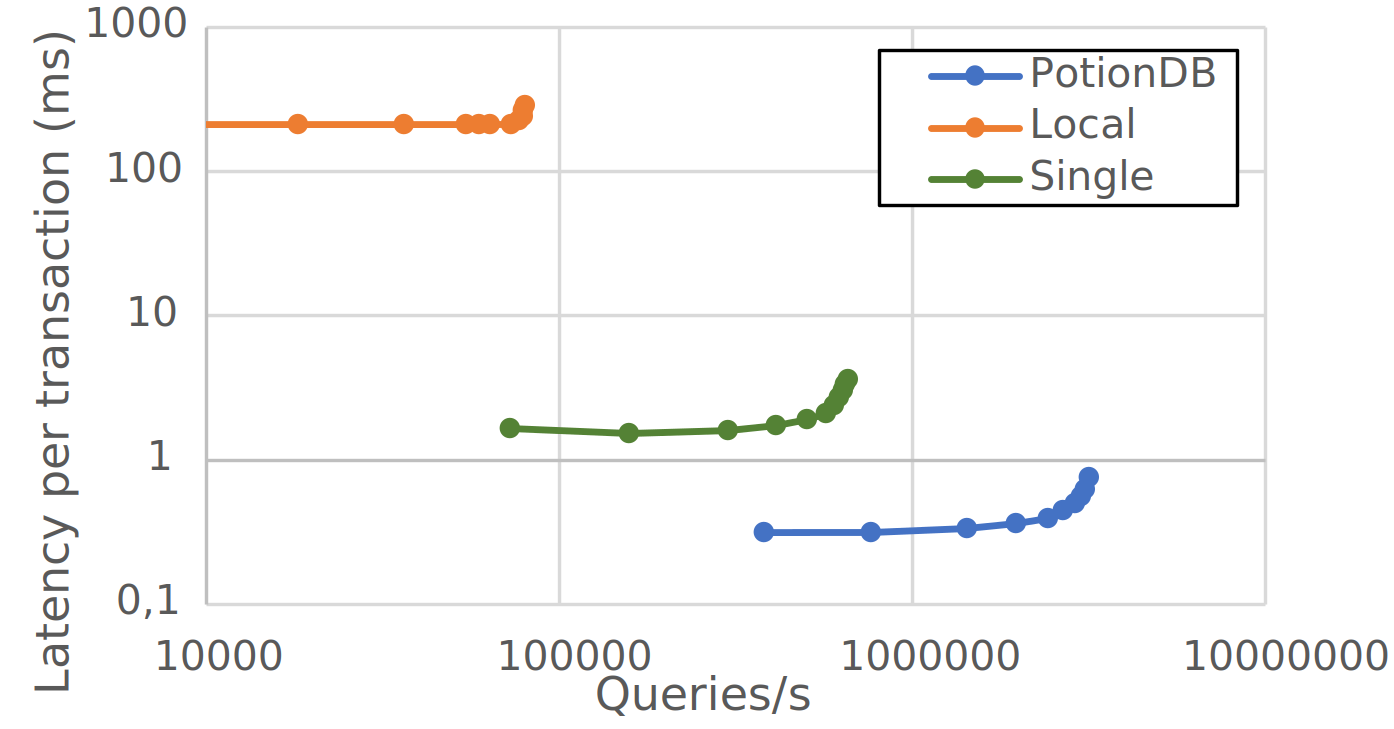
\includegraphics[width=1\linewidth]{clientScale_tc_cut}
		\caption{[OLD]PotionDB's performance executing all queries. (1txn = all queries (6 queries, 7 reads total)). Here the local PotionDB only scales up to around 80k ops/s and then starts increasing latency with no gain in throughput. Base latency is ~210ms (RTT to most distant server) as both local and global transactions are batched together.}
		\label{fig:(old)global_local_single_tc}
	\end{subfigure}
	\caption{}
\end{figure}

\subsection{Locality of data/Effects of data locality}

\begin{figure}[h]
	\centering
	\begin{subfigure}{.47\linewidth}
		\includegraphics[width=1\linewidth]{singleQuery/q3_latency}
		\caption{Query-only performance of Q3, a query of world-wide data. Base latency is 210ms (RTT to most distant server). For local PotionDB, after around 17k queries/s the latency starts rising, but throughput keeps rising albeit slower. I do not have an explanation to why throughput still keeps rising. (it even reaches 40k queries/s at 500ms latency with 20000 clients). PotionDB and Single have less throughput compared to old tests as there is no batching of queries (old version does 7 instances of Q3 per transaction). Likely the network overhead/protobuf overhead/base RTT is too much.}
		\label{fig:(new)q3_tc}
	\end{subfigure}%
	\hspace*{3em}
	\begin{subfigure}{.47\linewidth}
		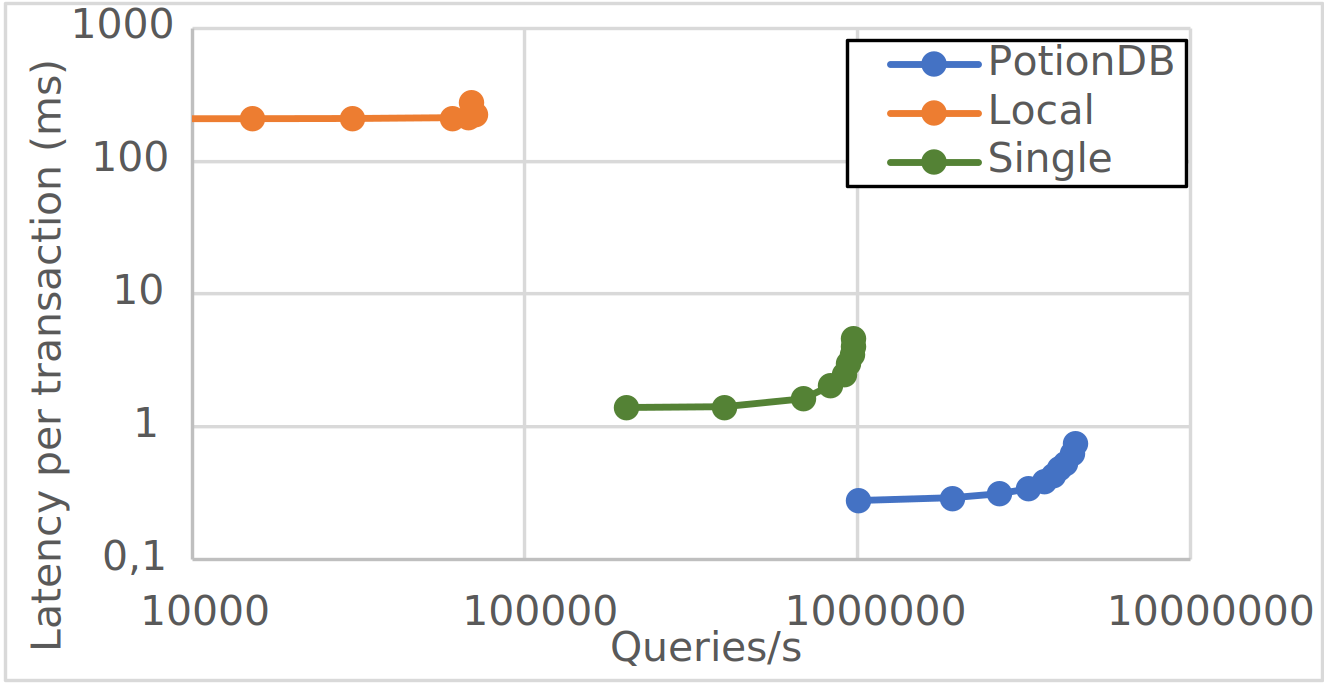
\includegraphics[width=1\linewidth]{Q3_tc}
		\caption{[OLD]Query-only performance of Q3, a query of world-wide data. Local PotionDB stops scaling at around 70k queries/s, going straight up in latency. This is a very logical result - servers saturate with the sheer amount of clients (at around 3000 clients).}
		\label{fig:(old)q3_tc}
	\end{subfigure}
	\caption{}
\end{figure}

\begin{figure}[h]
\centering
	\begin{subfigure}{.47\linewidth}
		\includegraphics[width=1\linewidth]{singleQuery/q5_latency}
		\caption{Query-only performance of Q5, a query of local data (data of a single region). Note that Local PotionDB is unaffected here by latency, as each instance can reply to clients' queries with only local views. Thus, Local PotionDB behaves like PotionDB. Single's throughput is about 1/5 of PotionDB as only one server can reply queries.}
		\label{fig:(new)q5_tc}
	\end{subfigure}%
	\hspace*{3em}
	\begin{subfigure}{.47\linewidth}
		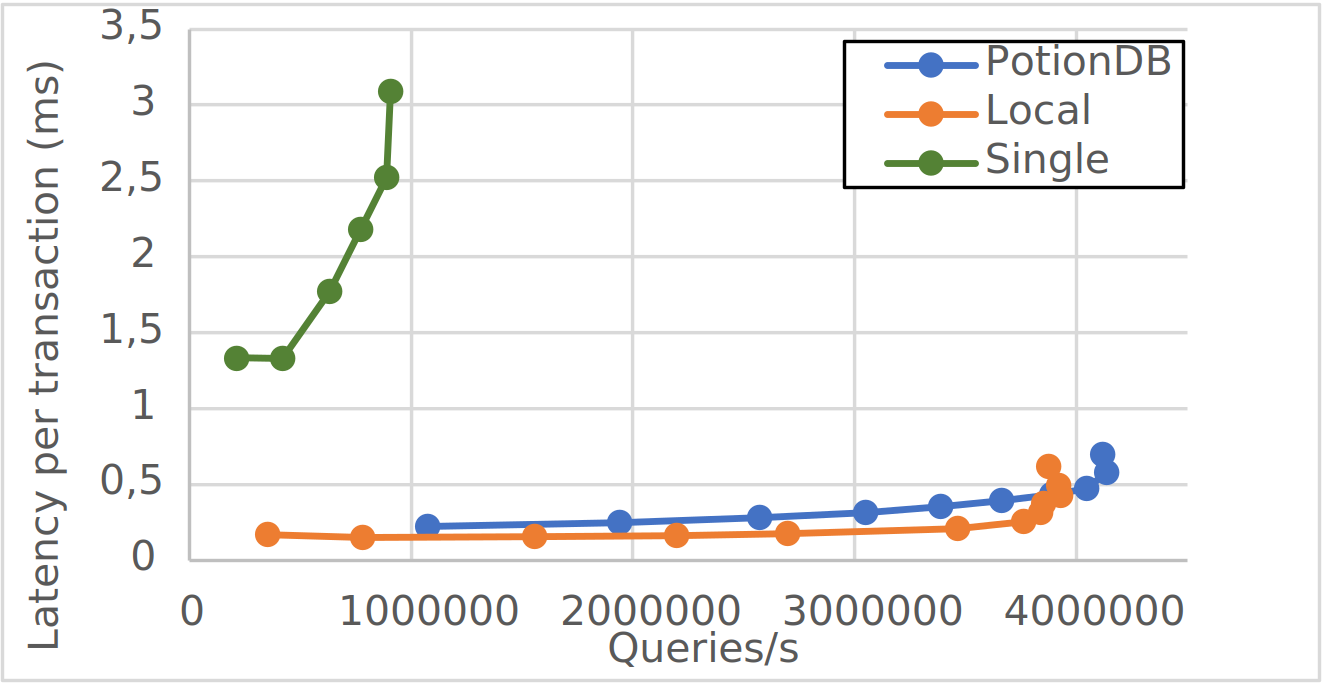
\includegraphics[width=1\linewidth]{Q5_tc}
		\caption{[OLD]Query-only performance of Q5, a query of local data (data of a single region). The higher throughputs compared to the new tests is simply due to the batching of queries.}
		\label{fig:(old)q5_tc}
	\end{subfigure}
\caption{}
\end{figure}

\subsection{PotionDB scaling with updates}

Note: Old graphs (Figures 4-6) still count index updates as updates. 
Index updates are about 40\% of all updates in non-local PotionDB.
Given queries are also factored in, the throughput in the old graphics would decrease very little except for 100\% updates (which we no longer want anyway).
For example, for 10\% updates, not counting with index updates is about less 4\% throughput.

\begin{figure}[h]
	\centering
	\begin{subfigure}{.47\linewidth}
		\includegraphics[width=1\linewidth]{singleQuery/upd_rate_global_noTC}
		\caption{PotionDB's performance with varying update rate. This graph already DOES NOT count with index updates for throughput. Adding updates does not hamper PotionDB as much as before due to multiple updates per txn: updates for an order + all its lineitems + all index updates (not counted but still executed); while queries now are individual (1 per txn). However, for 25\% updates, the effect is still noticeable as eventually there's too many update transactions going on, which leads to a lot of commits and synchronization between partitions.}
		\label{fig:(new)update_rates}
	\end{subfigure}%
	\hspace*{3em}
	\begin{subfigure}{.47\linewidth}
		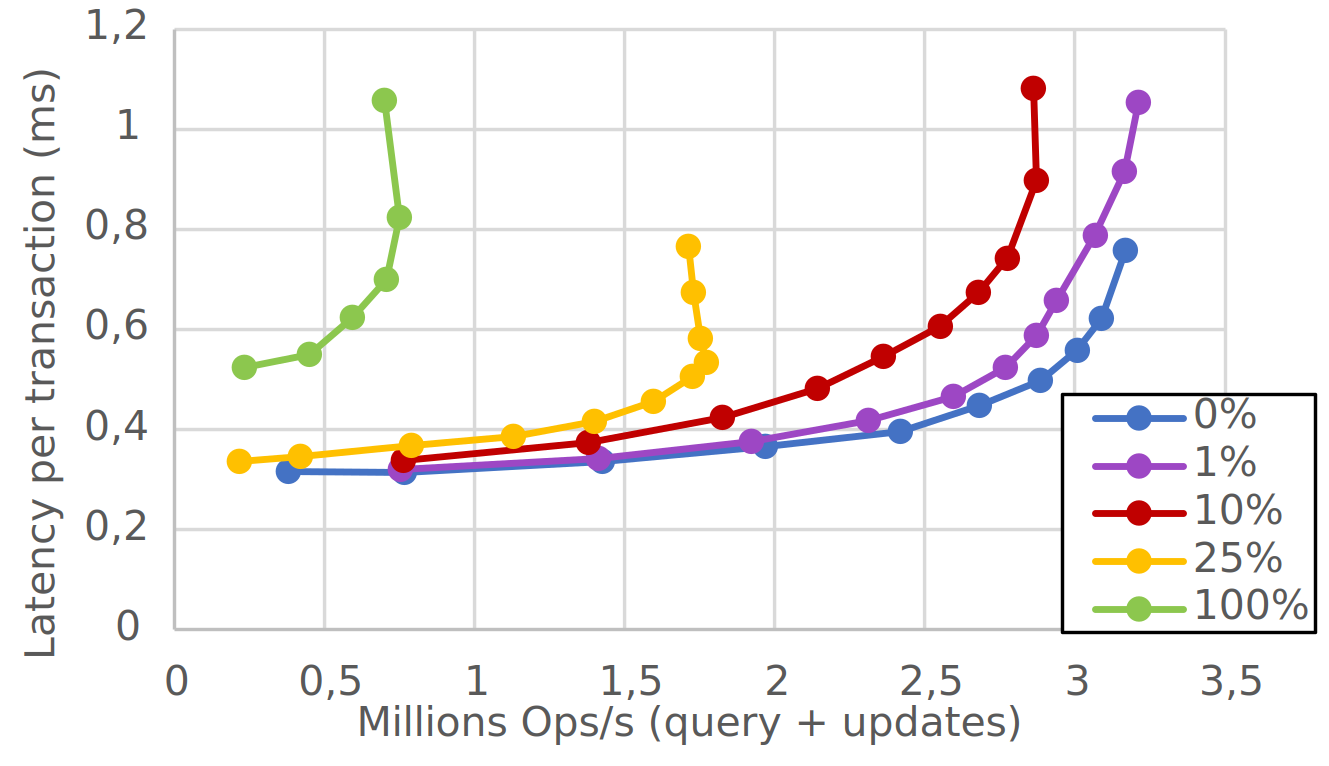
\includegraphics[width=1\linewidth]{updRate_global_cut}
		\caption{[OLD]PotionDB's performance with varying update rate. When multiple queries are executed per transaction, the effect of updates being slower is more noticeable.}
		\label{fig:(old)update_rates}
	\end{subfigure}
	\caption{}
\end{figure}

\begin{figure}[h]
	\centering
	\begin{subfigure}{.47\linewidth}
		\includegraphics[width=1\linewidth]{singleQuery/upd_rate_local_tc}
		\caption{Local PotionDB's performance with varying update rate. This graph already DOES NOT count with index updates for throughput. Results are similar all across - adding updates actually increases throughput slightly, due to batching. It seems difficult to reach a scalability cap - 48000 clients was not enough to fully saturate the servers, except for 25\% updates. Similar results to doing query-only: scales without latency increase until a certain point (25-32.5k ops/s depending on update ratio); afterwards throughput increase is slower and paired with latency increase.}
		\label{fig:(new)update_rates_local_tc}
	\end{subfigure}%
	\hspace*{3em}
	\begin{subfigure}{.47\linewidth}
		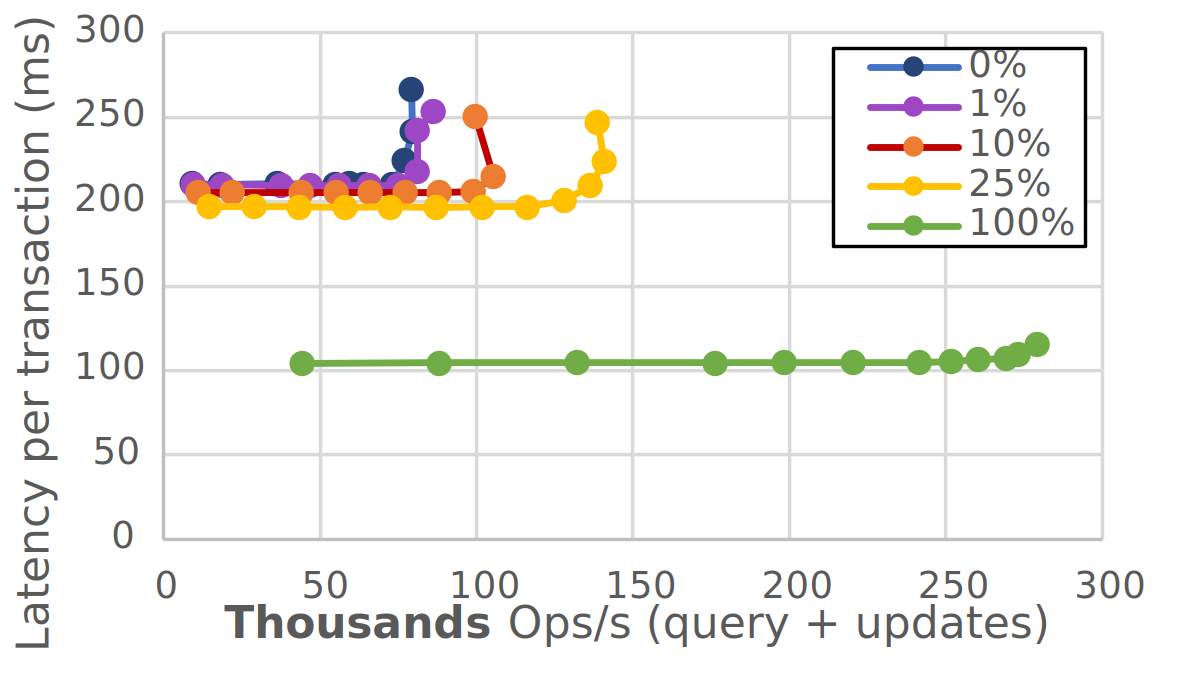
\includegraphics[width=1\linewidth]{updRate_tc_cut}
		\caption{[OLD]Local PotionDB's performance with varying update rate. Throughput increases until a certain point, then latency raises and throughput remains stable or even decreases a bit. The batching of queries lets throughput increase further before the latency is affected. Here the max throughput raising with updates is more noticeable, as less clients are needed to saturate the servers (thousands of clients instead of tens of thousands).}
		\label{fig:(old)update_rates_local_tc}
	\end{subfigure}
	\caption{}
\end{figure}


NOTE: THE TWO GRAPHICS IN FIGURES \ref{fig:(new)update_rates_single_tc}, \ref{fig:(old)update_rates_single_tc} WERE NOT IN THE PAPER BEFORE - and they probably shouldn't be now here. They're here for completude's sake, please tell me if you believe I should put them in the paper.

\begin{figure}[h]
	\centering
	\begin{subfigure}{.47\linewidth}
		\includegraphics[width=1\linewidth]{singleQuery/upd_rate_single_tc}
		\caption{(Note: This graphic wasn't present before in the paper.) Single PotionDB's performance with varying update rate. Mostly is about 1/5th of PotionDB, except for 25\%: the drop here in performance is less noticeable (here it is about 10\% less throughput, on PotionDB is about 25\% less throughput). At a first glance I do not know the why of this difference.}
		\label{fig:(new)update_rates_single_tc}
	\end{subfigure}%
	\hspace*{3em}
	\begin{subfigure}{.47\linewidth}
		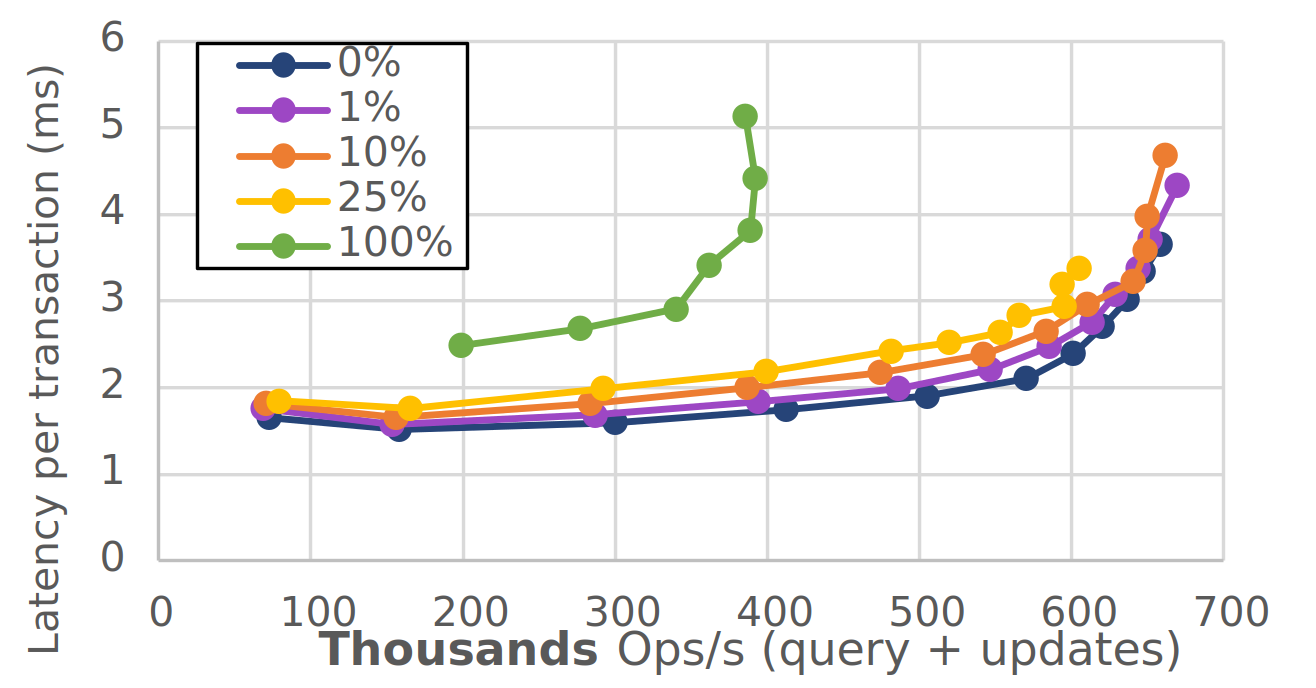
\includegraphics[width=1\linewidth]{upd_rate_tc_single}
		\caption{[OLD](Note: This graphic wasn't present before in the paper.) Single PotionDB's performance with varying update rate. Here the update rate also barely affects the throughput... I hadn't noticed this before. Oups. General throughput is higher compared to the new graph because of query batching, which saturates the view server with few clients.}
		\label{fig:(old)update_rates_single_tc}
	\end{subfigure}
	\caption{(NEW)}
\end{figure}

\subsection{PotionDB performance on a single DC}

\begin{figure}[h]
	\centering
	\begin{subfigure}{.47\linewidth}
		\includegraphics[width=1\linewidth]{singleQuery/all_queries_noTC}
		\caption{[NEW]Performance of all queries. Single PotionDB performs at about 1/5th of the throughput of PotionDB, as expected. Local PotionDB is quite slower due to 2/3rd of the queries requiring data to be gathered from all servers, adding extra latency, extra data transferred between servers and more requests processed per server.}
		\label{fig:(new)global_local_single_noTC}
	\end{subfigure}%
	\hspace*{3em}
	\begin{subfigure}{.47\linewidth}
		\includegraphics[width=1\linewidth]{singleQuery/q3_q5_noLatency}
		\caption{[NEW]Performance of Q3 and Q5. In PotionDB, Q3 only slightly underperforms Q5 (top 10 vs multiple counters transferred). Q5 local performs similarly to Q5 PotionDB, but Q3 Local underperforms considerably due to having to gather data from all servers to answer a single query.}
		\label{fig:(new)q3_q5_noTC}
	\end{subfigure}
	\caption{[NEW]Query-only performance of PotionDB and its local and single versions, without added latency. On the left all queries are executed, while on the right only Q3 (world-wide data) and Q5 (data local to a region) are.}
\end{figure}

\begin{figure}[h]
	\centering
	\begin{subfigure}{.47\linewidth}
		\centering
		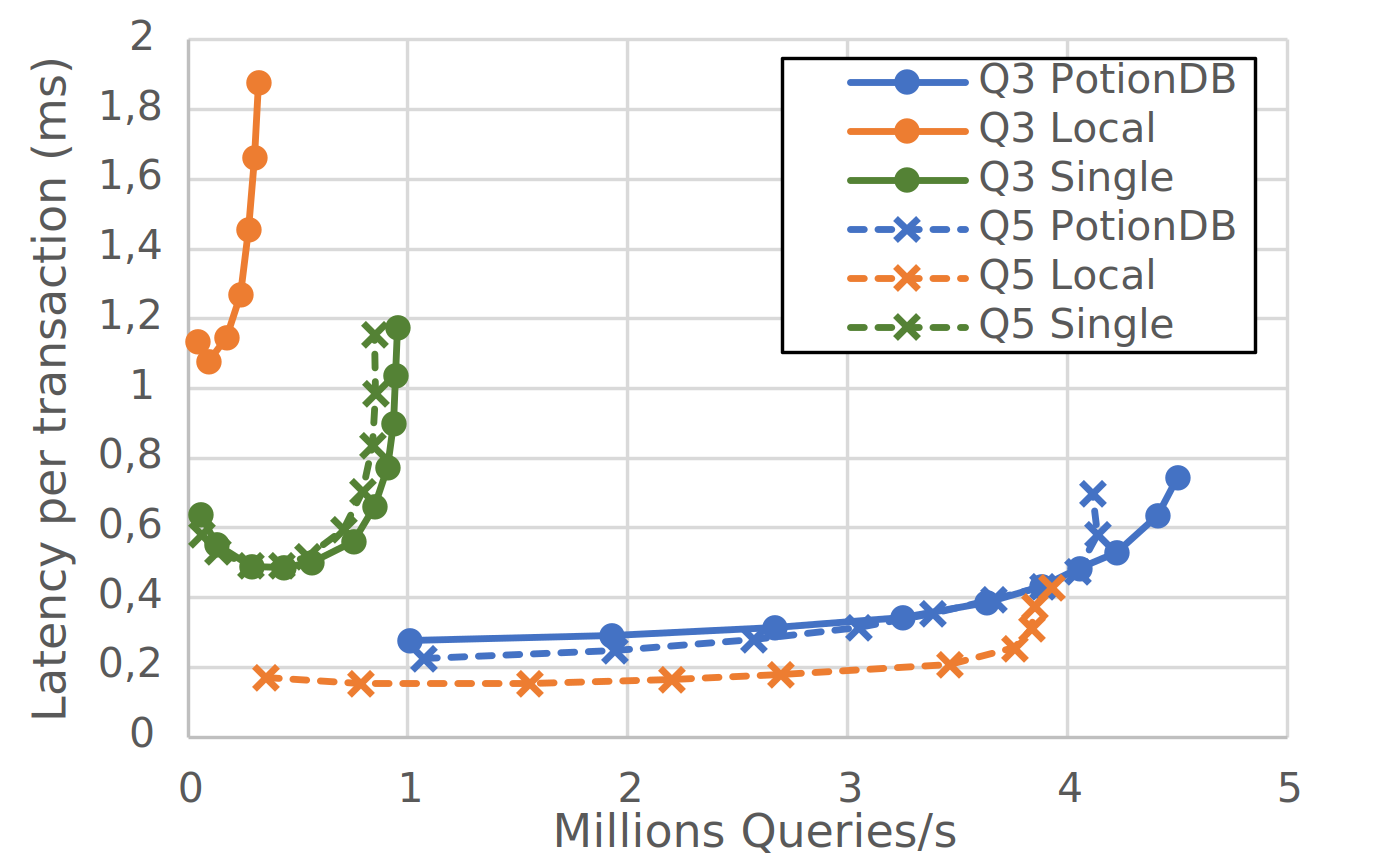
\includegraphics[width=1\linewidth]{clientScale_cut}
		\caption{[OLD]All queries. Similar to what is obtained in the new data, except with lower max throughputs due to query batching. Scaling here is more smooth too but latencies start higher.}
		\label{fig:(old)global_local_single}
	\end{subfigure}%
	\hspace*{3em}
	\begin{subfigure}{.47\linewidth}
		\centering
		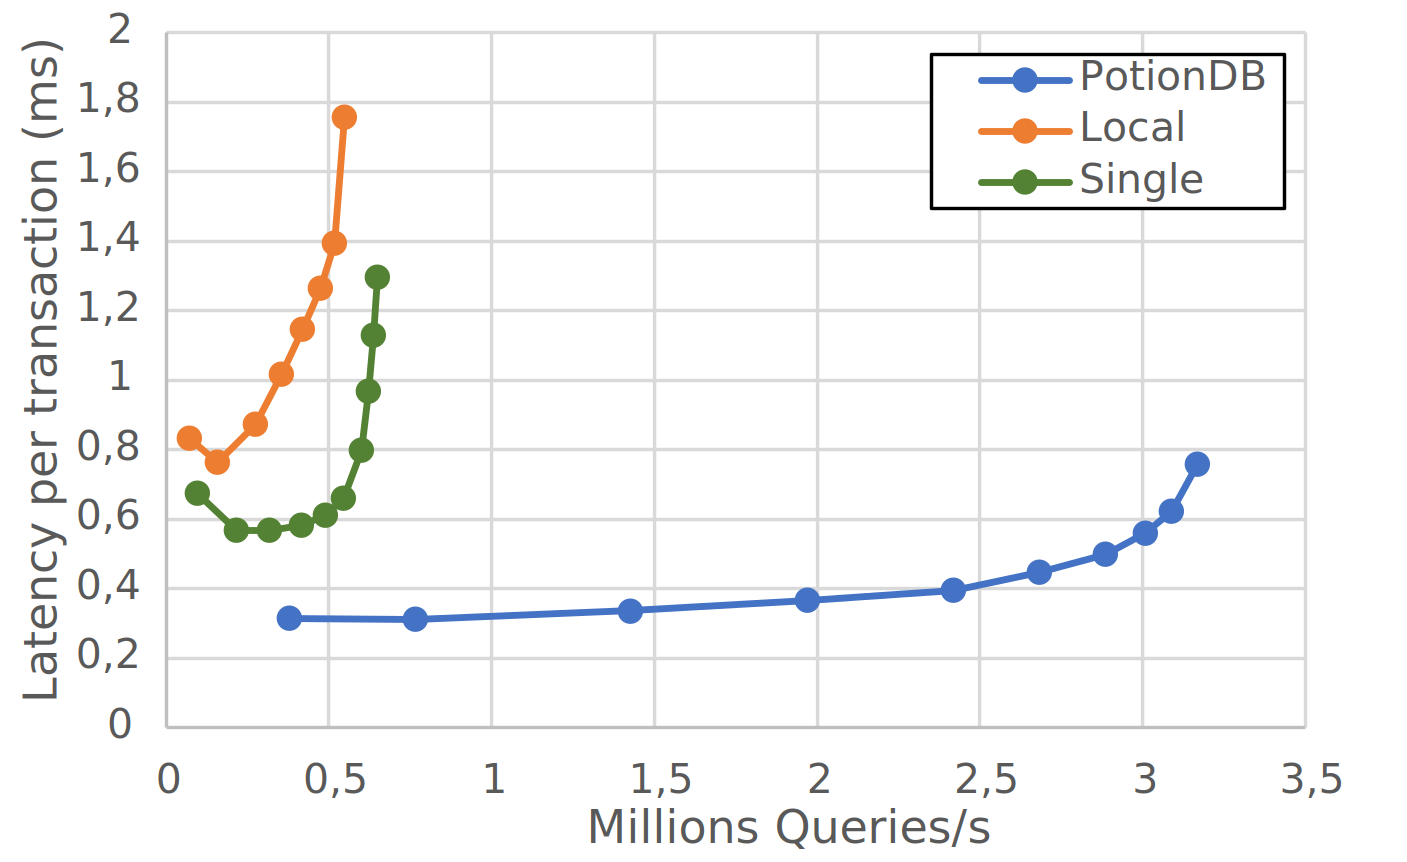
\includegraphics[width=.9\linewidth]{Q3vsQ5_cut}
		\caption{[OLD]Single query type. Similar to old data, but with PotionDB scaling quite further, specially on Q3. Here for PotionDB Q3 does better than Q5, unlike in the new data. I believe due to the structuring of protobufs - Q5 always returns multiple objects (counters), while Q3 only returns one (top10). Local here loses even more to PotionDB compared to the new data, due to too much data being transferred around to answer each query, which does not let it benefit from batching as much.}
		\label{fig:(old)q3q5}
	\end{subfigure}
	\caption{[OLD]Query-only performance of PotionDB and its local and single view versions, without added latency. On the left all queries are executed, while on the right only Q3 or Q5 are.}
	\label{fig:(new)query_only}
\end{figure}

\begin{figure}[h]
	\centering
	\begin{subfigure}{.47\linewidth}
		\includegraphics[width=1\linewidth]{singleQuery/upd_rate_global_noTC}
		\caption{}
		\label{fig:(new)(repeat)update_rates}
	\end{subfigure}%
	\hspace*{3em}
	\begin{subfigure}{.47\linewidth}
		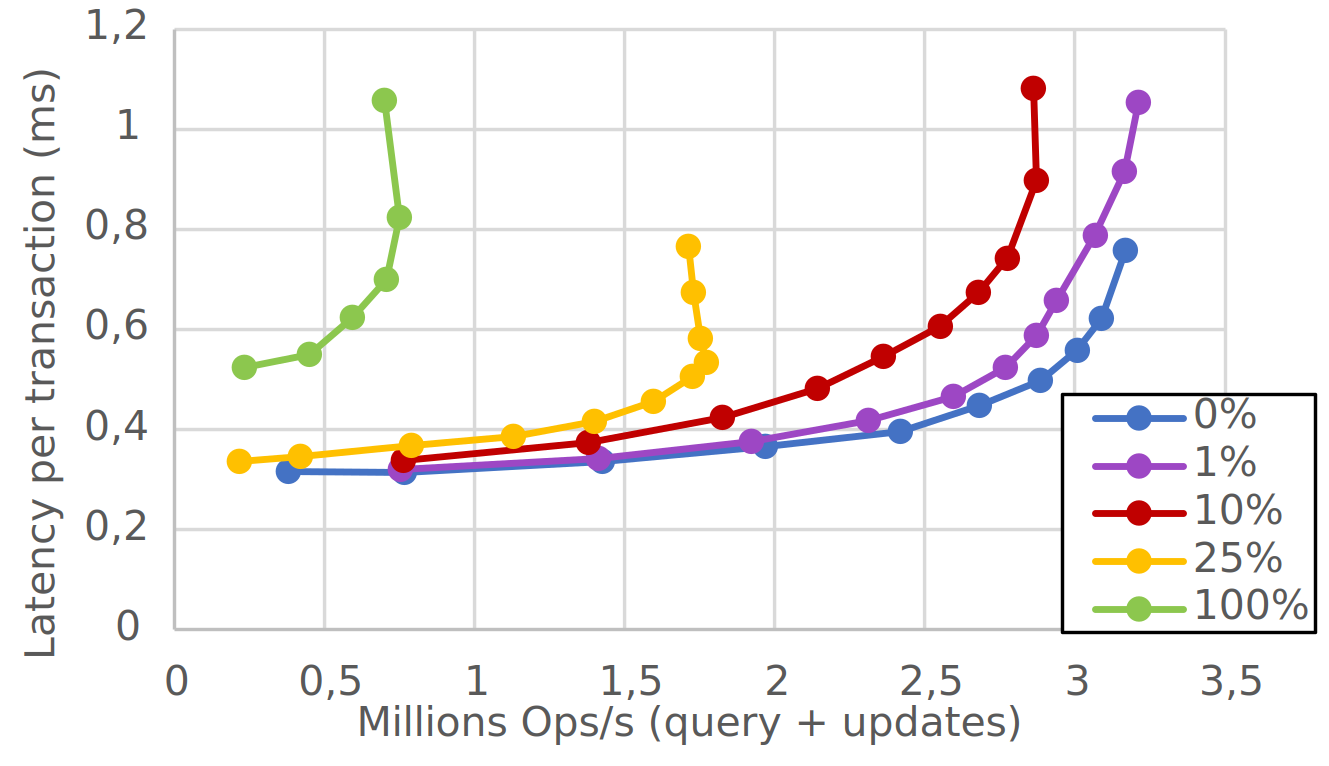
\includegraphics[width=1\linewidth]{updRate_global_cut}
		\caption{}
		\label{fig:(old)(repeat)update_rates}
	\end{subfigure}
	\caption{Yes, this is repeated. The idea is to show latency really does not make any difference, even with updates :)}
\end{figure}

\begin{figure}[h]
	\centering
	\begin{subfigure}{.47\linewidth}
		\includegraphics[width=1\linewidth]{singleQuery/query_latency_global_noTC}
		\caption{[NEW]Query-latency}
		\label{fig:(new)query_latency_noTC}
	\end{subfigure}%
	\hspace*{3em}
	\begin{subfigure}{.47\linewidth}
		\includegraphics[width=1\linewidth]{singleQuery/upd_latency_global_noTC}
		\caption{[NEW]Update-latency}
		\label{fig:(new)update_latency_noTC}
	\end{subfigure}
	\caption{[NEW](NOTE: are these graphics still relevant? My intention is to differentiate how the latency of queries/updates scale) PotionDB's performance with varying update rate, with query and update latencies split. Note that each query is its own transaction, while each update transaction has multiple updates - a new order, all associated items and all required view updates.}
\end{figure}

\begin{figure}[h]
	\centering
	\begin{subfigure}{.47\linewidth}
		\centering
		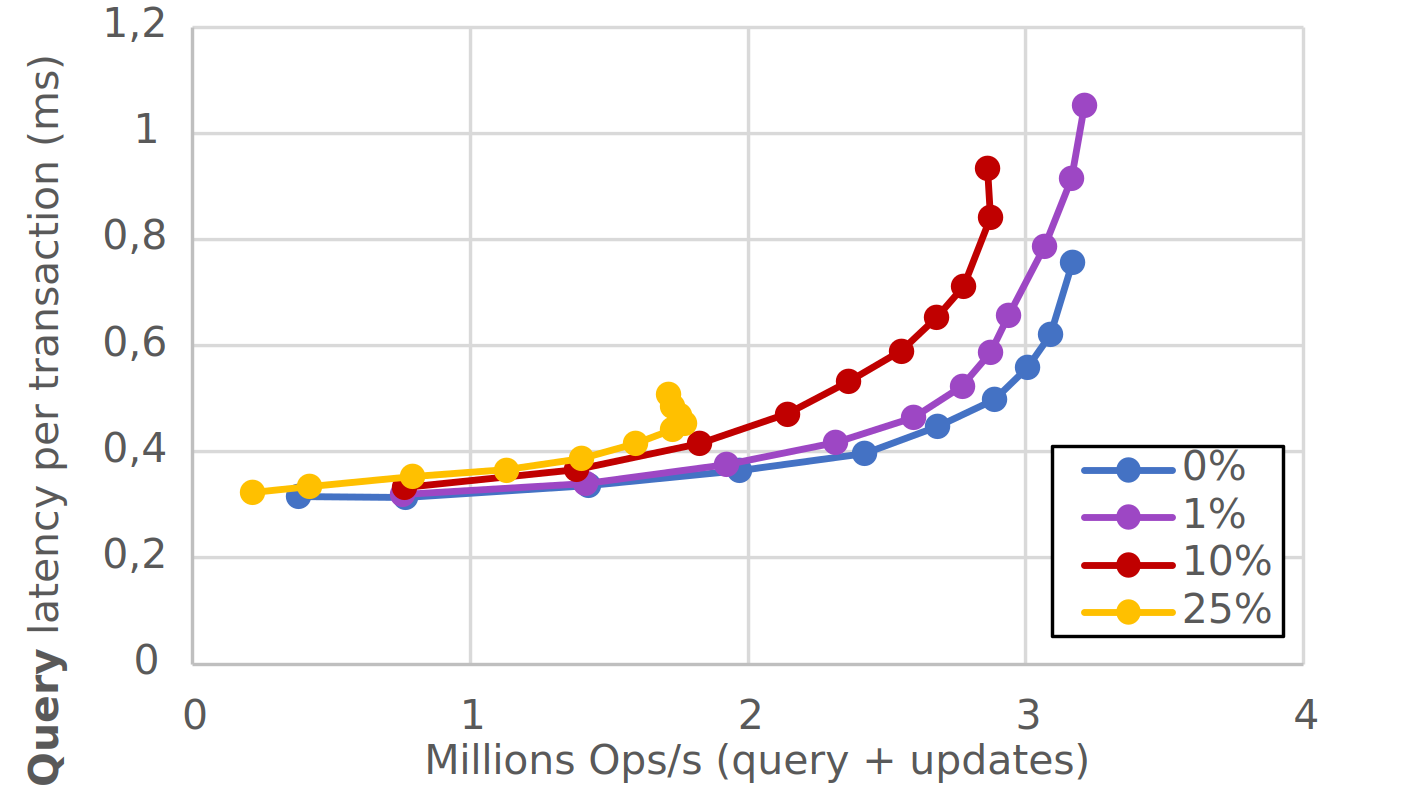
\includegraphics[width=1\linewidth]{updRate_queryLatency_cut}
		\caption{[OLD]Query-latency}
		\label{fig:(new)update_rates_query}
	\end{subfigure}%
	\hspace*{3em}
	\begin{subfigure}{.47\linewidth}
		\centering
		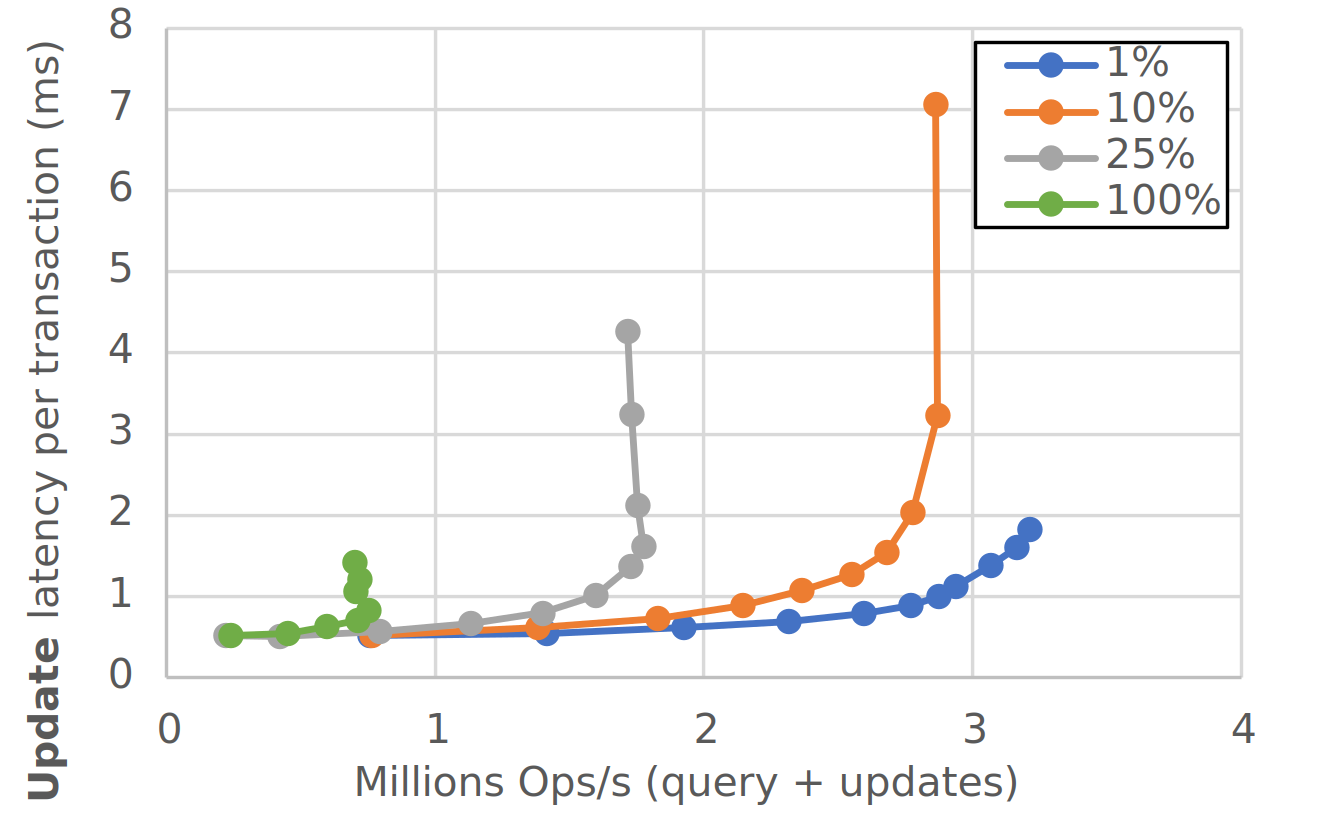
\includegraphics[width=1\linewidth]{updRate_updateLatency_cut}
		\caption{[OLD]Update-latency}
		\label{fig:(new)update_rates_update}
	\end{subfigure}
	\caption{[OLD]In terms of differences with the new data, not much worth saying. Query latencies start lower on new data due to being 1 query per txn. On both new and old data, update latencies suddenly spike (too many commits trying to happen simultaneously).}
	\label{fig:(new)update_rates_split}
\end{figure}

\begin{figure}[h]
	\centering
	\begin{subfigure}{.47\linewidth}
		\includegraphics[width=1\linewidth]{singleQuery/upd_rate_noTC_global_vs_local}
		\caption{[NEW]Normal(P\_) and Local (L\_) PotionDB's performance with varying update rate. With the new data, the throughput stays similar for all update rates on local PotionDB, with there only being a very slight difference/variance when maxing the throughput. Even the latencies are extremely similar. Note that index updates are not counted here for throughput.}
		\label{fig:(new)update_rates_global_vs_local}
	\end{subfigure}%
	\hspace*{3em}
	\begin{subfigure}{.47\linewidth}
		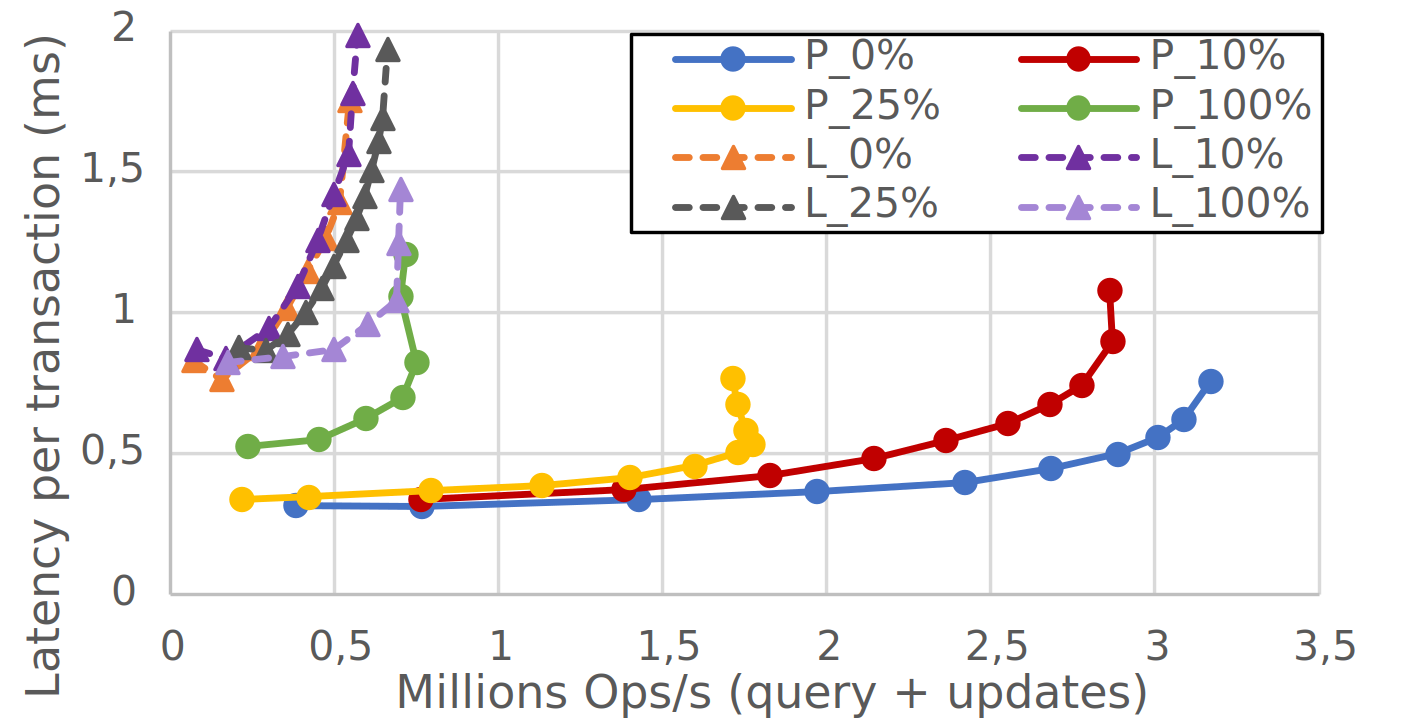
\includegraphics[width=1\linewidth]{updRate_localvsglobal_cut}
		\caption{[OLD]Normal(P\_) and Local (L\_) PotionDB's performance with varying update rate. Here updates on local increase throughput slightly. Importantly this is still counting with index updates - not counting with them would bring the throughputs slightly closer (40\% of all updates are index updates), but I believe the throughput would still rise slightly with the update rate.}
		\label{fig:(old)update_rates_global_vs_local}
	\end{subfigure}
	\caption{}
\end{figure}

\subsection{Types of views (or maybe, Views type benchmarking?)}

Note: Need suggestions for the title above.
IMPORTANT NOTE: I am thinking of doing batching here for the top sizes, as otherwise no difference is observable between top 1, top 10 and top 100 - I can always make bigger top sizes, but that doesn't make much sense.
I will either do batches of 10, 7 (the value used in the old data) or 5.

\begin{figure}[h]
	\centering
	\begin{subfigure}{.47\linewidth}
		\includegraphics[width=1\linewidth]{singleQuery/bench_top_size_0_upd}
		\caption{[NEW]TopK query performance with a varying top size. Sadly nothing observable for top1 - top100 when executing transactions of only 1 query: too much overhead on other things. Top 1000 has much less throughput - data transferred starts to matter. Noticeably, due to only being 1 query instead of 7, latencies for top 1000 and 100 are much lower when compared to the old data.}
		\label{fig:(new)bench_top_size_0upd}
	\end{subfigure}%
	\hspace*{3em}
	\begin{subfigure}{.47\linewidth}
		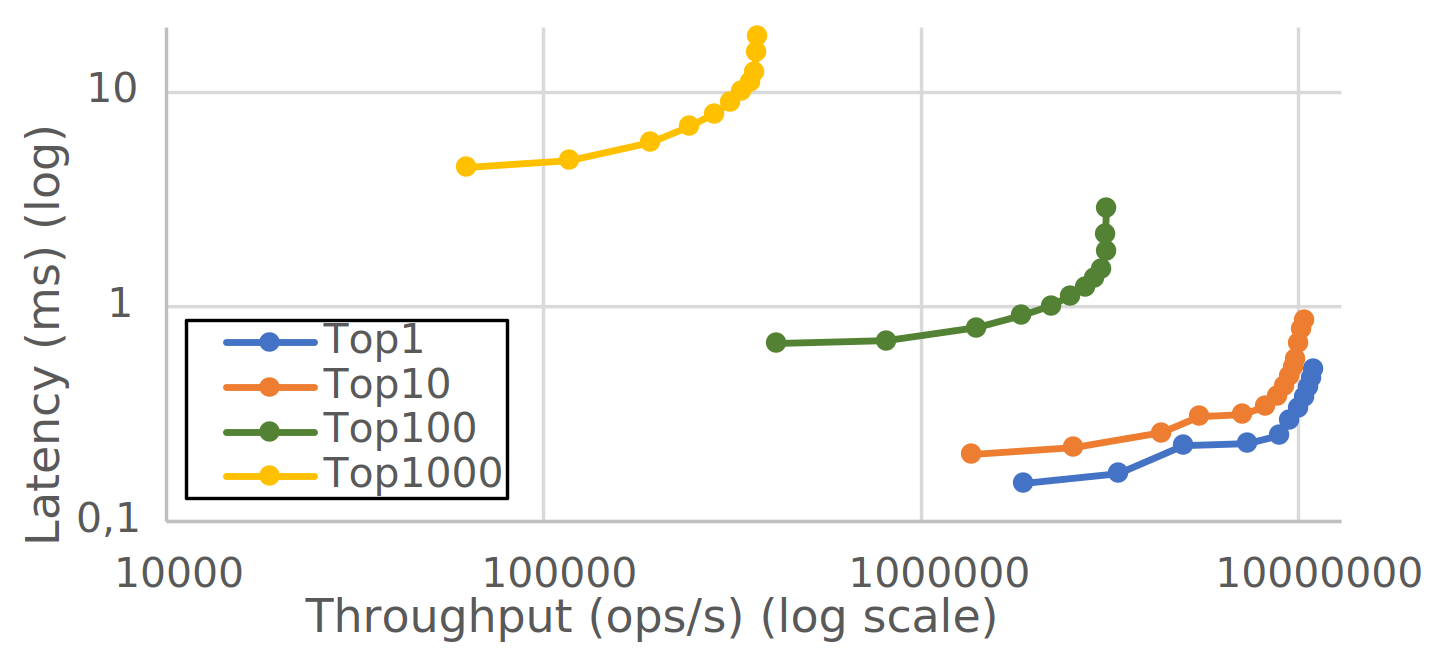
\includegraphics[width=1\linewidth]{TopKTopSize0upd_cut}
		\caption{[OLD]TopK query performance with a varying top size. Top 1 and Top 10 are somewhat similar - the amount of data transferred is small compared to communication overhead + cost of serialization/deserialization of protobufs, as well as high number of clients handled at a time. 10 -> 100 and 100 -> 1000 decrease by, respectively, 70\% and 88\%: the amount of data transferred is what matters most. After 1000, a linear decrease would be expected.}
		\label{fig:(old)bench_top_size_0upd}
	\end{subfigure}
	\caption{}
\end{figure}

\begin{figure}[h]
\centering
\begin{subfigure}{.47\linewidth}
	\includegraphics[width=1\linewidth]{singleQuery/bench_top_size_0_1}
	\caption{[NEW]Performance with 10\% updates, 90\% reads. Max throughput decreases considerably. Top1-100 has same query performance - I just need to scale Top1-10 to the same clients as Top100. Nothing interesting to really observe. (Note: this upd rate was not tested with the old data)}
	\label{fig:(new)bench_top_size_0_1upd}
\end{subfigure}%
\caption{}
\end{figure}

\begin{figure}[h]
	\centering
	\begin{subfigure}{.47\linewidth}
		\includegraphics[width=1\linewidth]{singleQuery/bench_top_size_0_25}
		\caption{[NEW]Performance with 25\% updates, 75\% reads. Max throughput decreases even more considerably. Max throughput for Top1000 increases - updates are lighter than the amount of data transferred on queries. Top 1-100 still have about the same performance (just need to test with more clients for Top 1-10.)}
		\label{fig:(new)bench_top_size_0_25upd}
	\end{subfigure}%
	\hspace*{3em}
	\begin{subfigure}{.47\linewidth}
		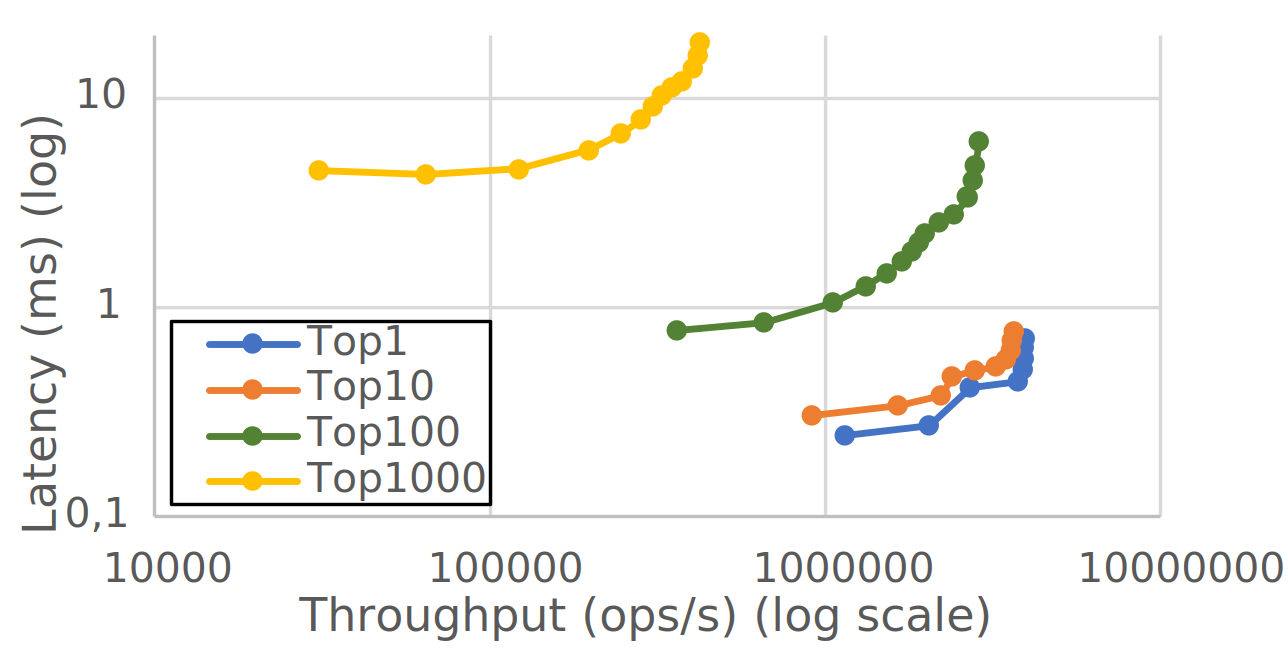
\includegraphics[width=1\linewidth]{TopKTopSize25upd_cut}
		\caption{[OLD]Performance with 25\% updates, 75\% reads. Max throughput for Top 1 and Top 10 decreases considerably, for Top 100 seems similar (but higher latency), for Top 1000 is a little bit higher.}
		\label{fig:(old)bench_top_size_0_25upd}
	\end{subfigure}
	\caption{}
\end{figure}

\begin{figure}[h]
	\centering
	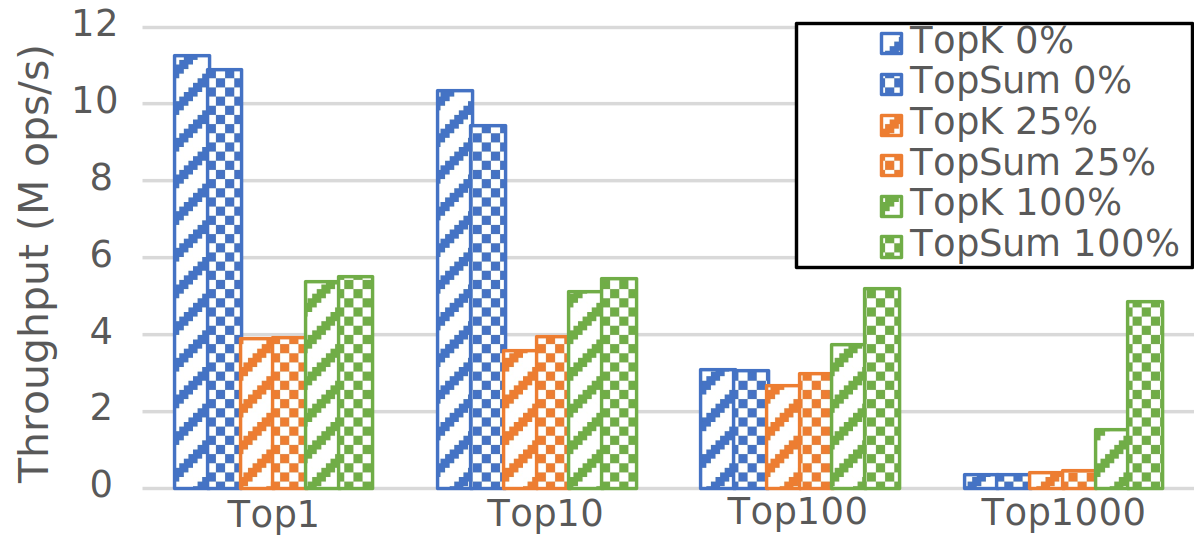
\includegraphics[width=.5\linewidth]{TopKVSTopSum_cut}
	\caption{[OLD GRAPHICS, I HAVE NOT DONE THE NEW ONE OF THIS (I do have the data already though)] (Note: the discrepancy between TopK and TopSum for high update rates should be gone on the new data). TopK and TopSum performances for different top sizes and update rates.}
	\label{fig:(new)TopkVSTopsum}
\end{figure}

\begin{figure}[h]
	\centering
	\begin{subfigure}{.33\linewidth}
		\centering
		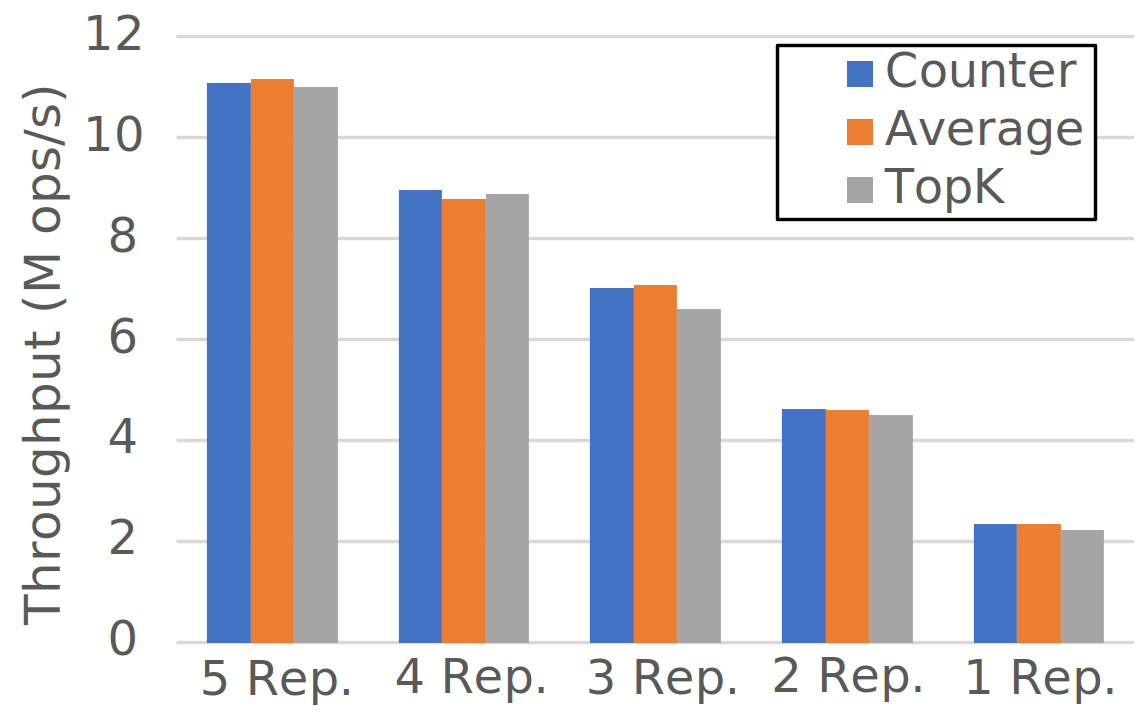
\includegraphics[width=.97\linewidth]{CounterAvgTopK0upd_v2_cut}
		\caption{0\% update rate}
		\label{fig:(new)CounterAvgTopK0upd}
	\end{subfigure}%
	\begin{subfigure}{.33\linewidth}
		\centering
		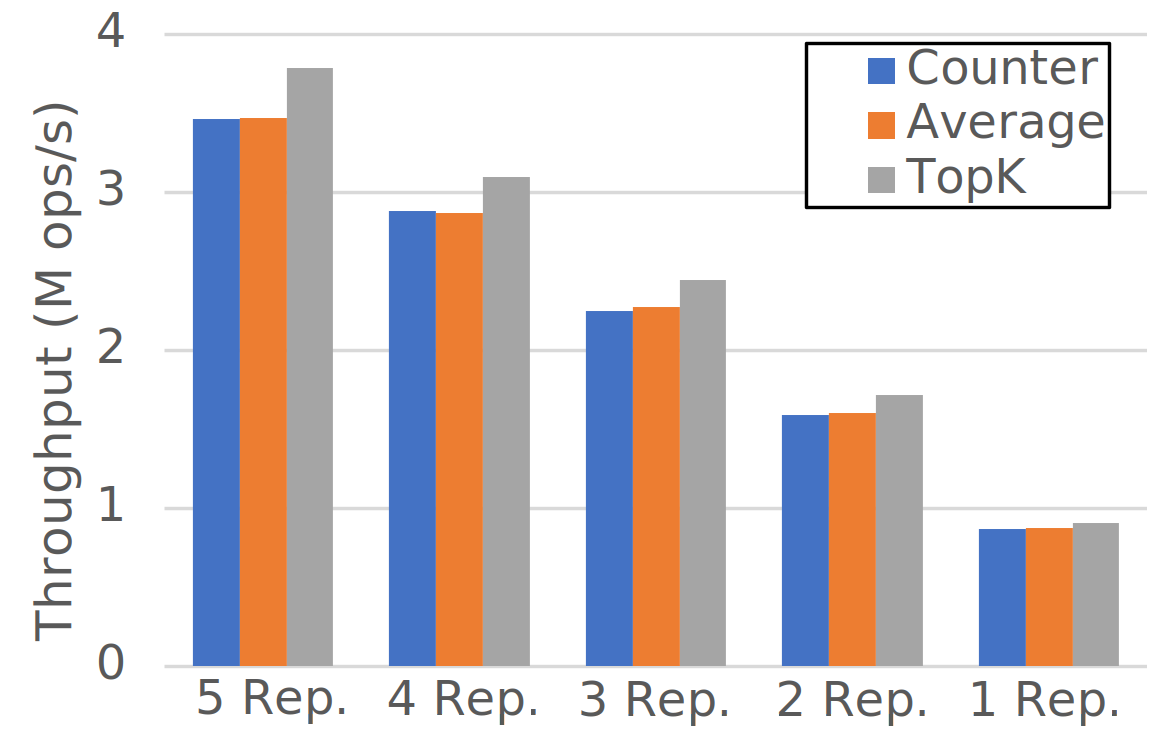
\includegraphics[width=.97\linewidth]{CounterAvgTopK25upd_v2_cut}
		\caption{25\% update rate}
		\label{fig:(new)CounterAvgTopK25upd}
	\end{subfigure}%
	\begin{subfigure}{.33\linewidth}
		\centering
		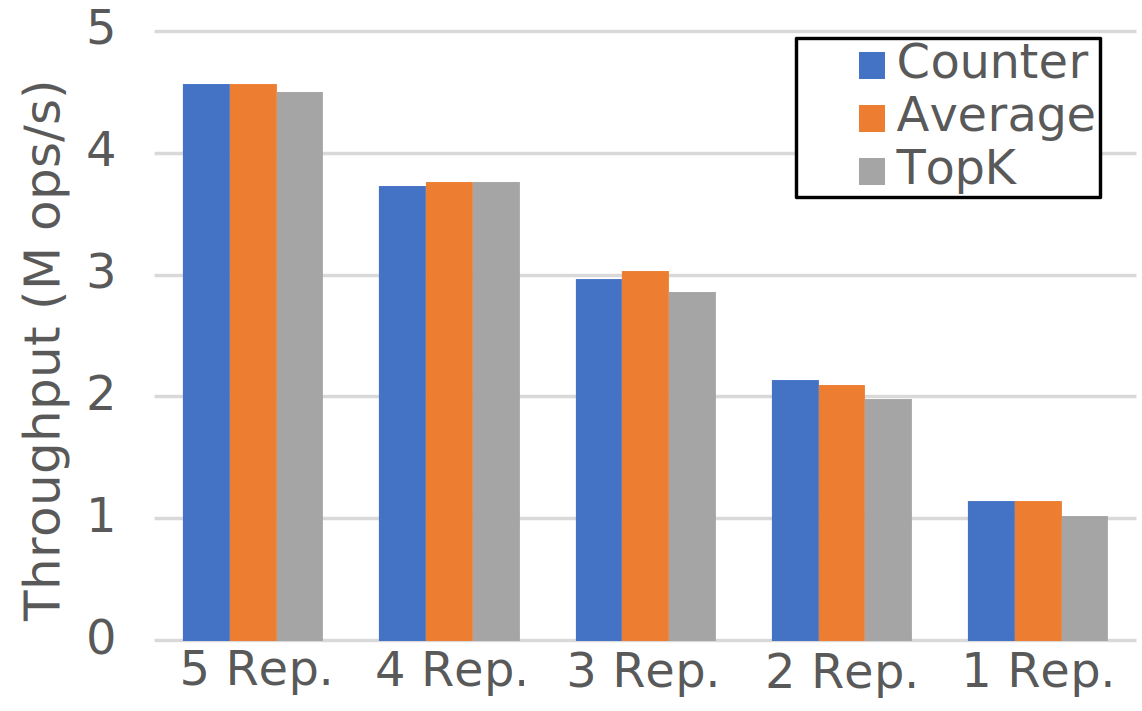
\includegraphics[width=.97\linewidth]{CounterAvgTopK100upd_v2_cut}
		\caption{100\% update rate}
		\label{fig:(new)CounterAvgTopK100upd}
	\end{subfigure}
	\caption{[OLD GRAPHICS, I HAVE NOT DONE THE NEW ONE OF THIS (I do have the data already though)] Counter, Average and TopK CRDTs performance for different numbers of replicas and update rates.}
	\label{fig:(new)CounterAvgTopK}
\end{figure}


\end{document}